\chapter{Apresentação da Concedente} % (fold)
\label{chap:Apresentação da Concedente}
Em \cite{CARVALHO:2012} orienta-se aos estagiários tomarem conhecimento do ambiente escolar primeiramente por intermédio da observação e da análise, buscando-se compreender a realidade em que se contra, bem como a relação da unidade escolar com a comunidade, dessa forma, pretende-se estabelecer a vivência pedagógica a partir da tomada de conhecimento de maneira humana e solidarizada.

\section{Caracterização da Unidade} % (fold)
\label{sec:Caracterização da Unidade}
\setlength\intextsep{0pt}
\begin{wrapfigure}[9]{r}{0.5\textwidth}
	\centering
	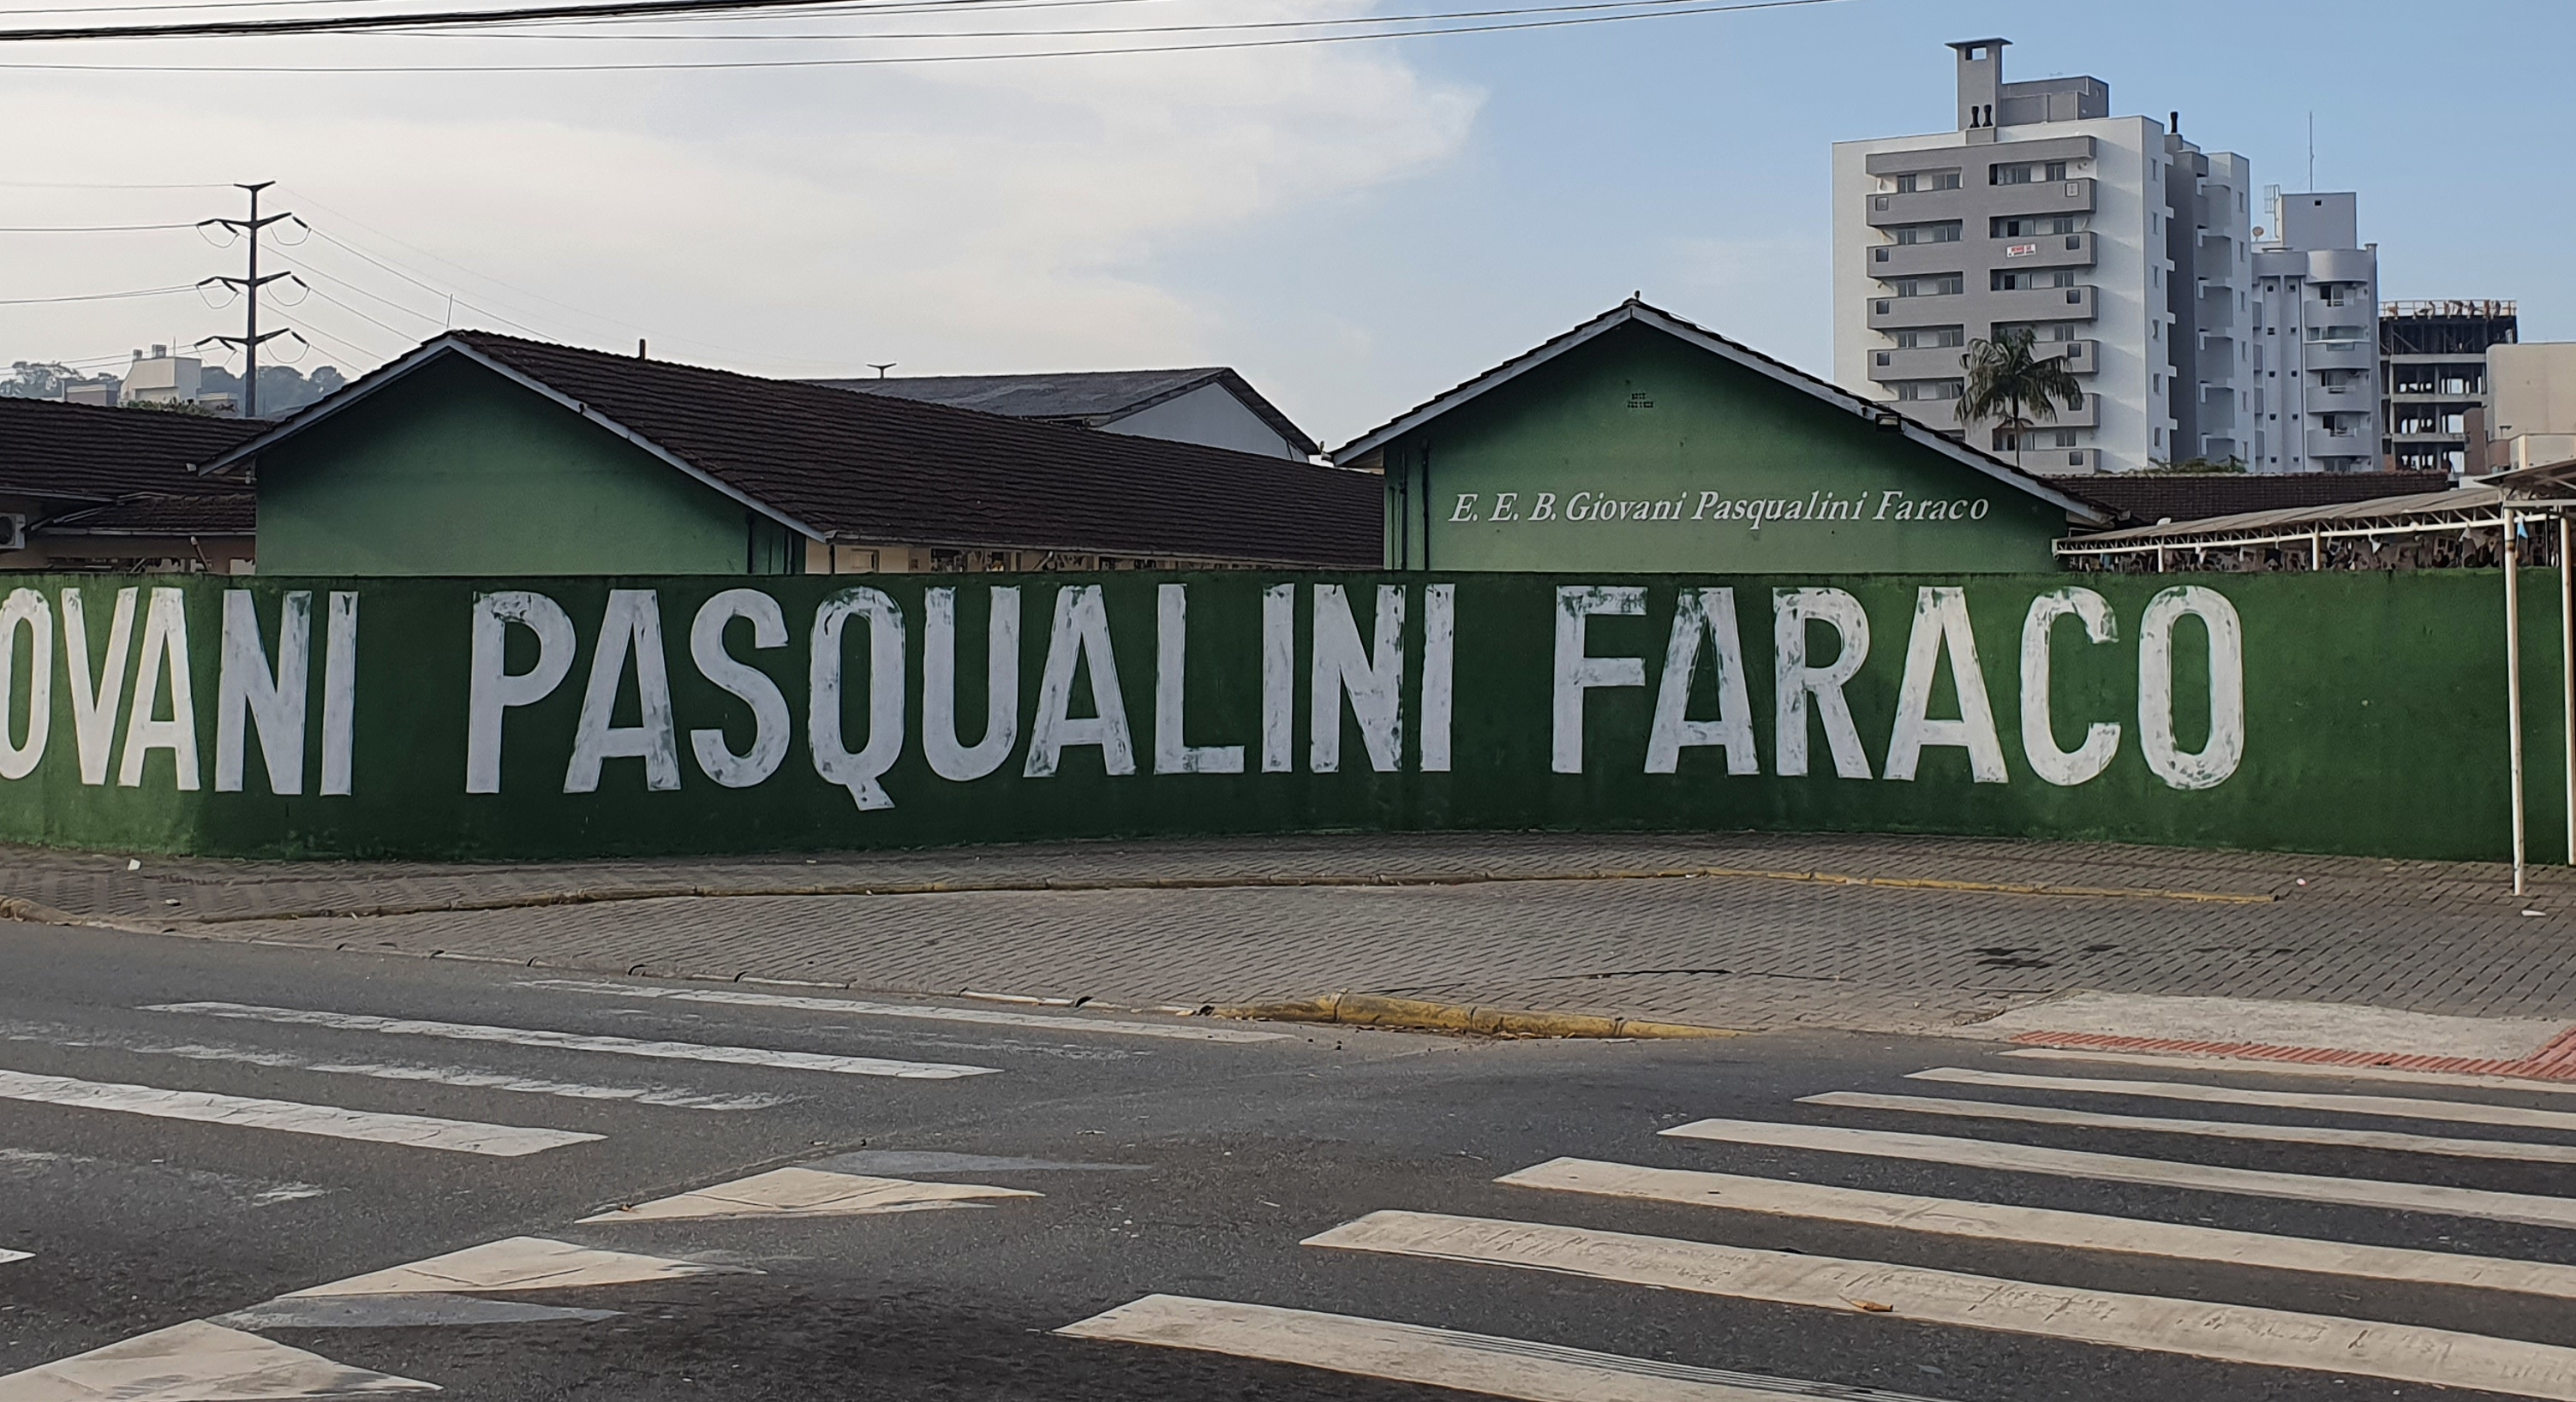
\includegraphics[width=.45\textwidth]{assets/vista-ext01.jpg}
	\label{fig:vista-externa}
	\caption{EEB-GPF: Visão externa.}
\end{wrapfigure}
A \ac{EEB} \ac{GPF} não se destingue do padrão estrutural das escolas pública de joinville, tal como outras tantas, mistura-se à paisagem urbana da região, no caso a região norte da cidade. Em tinta branca e em caixa alta é lido o nome da escola numa parte do muro e, dessa forma, os muros não apenas lhe conferem \emph{proteção}, mas também referência.

\setlength\intextsep{0pt}
\begin{wrapfigure}[15]{l}{0.5\textwidth}
	\centering
	\includegraphics[width=.45\textwidth]{assets/entrada-01.jpg}
	\label{fig:entr-principal}
	\caption{EEB-GPF: Entrada principal}
\end{wrapfigure} A entrada principal, consiste num portão largo, aberto ao início e final de cada turno, é por onde passam a maioria dos alunos, um segundo portão feito de grade e estreito é visto mais adiante, este da acesso à secretaria. Sempre de clima agradável, bem equipada e limpa, a secretaria é a primeira instância administrativa de que a comunidade tem acesso direto à escola, há sempre alguém de prontidão e não demora muito a atendê-lo. Folhetos no balcão e cartazes colados nos murais, informam as datas e atividades que a escola desenvolve em conjunto com a comunidade. Um caminho estreito e florido, liga a secretaria ao hall onde ficam as salas: do(a) \ac{ATP}, da Direção Geral, e dos Professores.

A unidade funciona nos três turnos disponíveis, atendendo desde o 1º ao 9º ano do \ac{EF}, do 1º ao 2º ano do \ac{NEM} e, pelo menos por enquanto, ao 3º ano do \ac{EM}.
% section Caracterização da Unidade (end)

\subsection{Histórico} % (fold)
\label{sec:Histórico}
Foi fundada no dia 15 de fevereiro de 1938 (85 anos) sob o nome: \textit{Escola Desdobrada Dona Francisca Quilômetro Cinco}. Encontra-se situada junto à Rua Dona Francisca, número 4957, Bairro Santo Antônio, região norte de Joinville-SC. 

Atualmente têm em seu nome o patrono da instituição: \emph{Giovani Faraco} -- brasileiro, nascido em 05 de abril de 1915, foi professor de latin, português e compositor de músicas para órgãos. O Decreto de n$^\circ$ 10138/70 renomeia a unidade para Grupo Escolar Giovani Pasqualini Faraco e em 08 de junho de 1993, recebe aprovação do Conselho Estadual de Educação para implantar o Ensino Médio através do parecer de n$^\circ$ 117/93, integrando desde então a rede Estadual de Ensino.
% subsection Histórico (end)

\subsection{Infraestrutura} % (fold)
\label{sec:Infraestrutura}

Tem por área construída  $3114,50\m^2$ e outros $13929,25\m^2$ de área disponível. Conta com uma infraestrutura de: 17 salas de aulas de $42\m^2$ cada, cozinha, depósito para merenda escolar, depósito para produtos de limpeza, cantina, banheiros feminino e masculino, banheiros para professores, biblioteca, laboratório para as disciplinas de Física/Química e Biologia, laboratório de informática, sala ambiente para a disciplina de língua Portuguesa, arquivo inativo, sala para materiais de Educação Física, sala para materiais e equipamentos de: orientação escolar, direção, vídeo, artes e materiais para docentes.

A área descoberta é limpa, agradável e bem cuidada, possui árvores ao seu redor criando um ambiente convidativo para o exercício da leitura, recreação ou até mesmo aulas diversificadas. Possui também uma pérgola onde se realizam aulas de leitura. Para um contato maior com a terra, dispõe de uma horta escolar, onde os alunos podem fazer o reconhecimento de hortaliças e vegetais.

Possui pátio e quadras cobertas, onde são feitas as atividades culturais e esportivas, além das refeições no horário do recreio.
% subsection Infraestrutura (end)

\subsection{Recursos Humanos} % (fold)
\label{sub:Recursos Humanos}
A equipe gestora da unidade é caracterizada pela Diretora e duas Assessoras que estão sempre disponíveis nas dependências do estabelecimento. Para a funcionalidade pedagógica e administrativa, conta com uma equipe técnica de Assistentes Técnicos(as) Pedagógicos(as) e Assistentes Educacionais, todos bem solícitos e acessíveis aos alunos, pais e estagiários.
% subsection Recursos Humanos (end)

\subsection{Perfil Socioeconômico} % (fold)
\label{sub:Perfil Socioeconômico}
\textcolor{red}{[REVISAR]}

É situada perto de empresas locais e centros educacionais como: UNIVILLE, SENAI, IFSC e UDESC. Os estudantes que compõem o corpo discente, em geral, são de famílias pertencente à classe média, 80\% de etnia branca, 10\% negras, 5\% pardos e indígenas e outros 5\% não declarados. As famílias são de religião predominantemente cristã em que 60\% são evangélicos, 25\% católicos, 5\% luteranos, 5\% de raiz africana e 5\% não declarados. Ocupam-se das mais variadas funções, distribuídas em 30\% autônomos, 40\% funcionários das indústrias da região, 15\% exercem atividades comerciais, 5\% prestam serviços e 10\% não declararam.

A maioria dos responsáveis pelas famílias concluiu o \ac{EM} e incentiva os filhos a ingressarem no Ensino Superior, acredita que a educação é a \emph{garantia de um futuro melhor}. 
% subsection Perfil Socioeconômico (end)

\subsection{Estatísticas} % (fold)
\label{sub:Estatísticas}
\textcolor{red}{[REVISAR E ATUALIZAR OS QUADROS]}

Realiza anualmente registros e análises dos principais índices da educação básica e busca implementar ações de melhoria através de reuniões de estudo e cursos de capacitação de professores. A seguir apresentamos três quadros resultantes destas ações. 
% subsection Estatísticas (end)

\section{Projeto Político Pedagógico} % (fold)
\label{sec:Projeto Político Pedagógico}
\textcolor{red}{[REVISAR E RESUMIR]}

Em \cite{CARVALHO:2012a}, o \ac{PPP} é um documento representativo do pensamento escolar, destaca a importância da elaboração deste documento em conjunto com a comunidade; pais, professores, representantes de alunos e equipe diretiva. Uma atenção ainda é dada a necessidade do documento manter-se disponível a todos os entes desta comunidade. 

Outro trabalho desenvolvido por \cite{VEIGA:1995} traz a consolidação do PPP como elemento resultante de uma ação intencional de sentido explícito e compromisso definido coletivamente,

\begin{citacao}
    ``\ldots todo projeto pedagógico de uma escola é, também, um projeto político por estar intimamente articulado ao compromisso sociopolítico com os interesses reais e coletivos da população majoritária. É político no sentido de compromisso com a formação do cidadão para um tipo de sociedade. A dimensão política se cumpre na medida em que ela se realiza como prática especificamente pedagógica. Na dimensão pedagógica reside a possibilidade da efetivação da intencionalidade da escola, que é a formação do cidadão participativo, responsável, compromissado, crítico e criativo. Pedagógico, no sentido de definir as ações educativas e as características necessárias às escolas de cumprirem seus propósitos e sua intencionalidade.'' \opcit[p. ~2]{VEIGA:1995}
\end{citacao}
Dessa forma entende-se que tanto o processo de construção quanto o a aprovação do \ac{PPP} deva seguir tais preceitos. Cabe ainda à gestão escolar providenciar formas de viabilizar a participação de todos os membros da comunidade escolar. 

\subsection{Atribuição dos Agentes}
A \ac{GPF} posiciona-se de acordo com estes referenciais ao prever em seu \ac{PPP}

\begin{citacao}
    ``\ldots A participação dos professores e especialistas na elaboração do projeto pedagógico promove uma dimensão democrática na escola e nessa perspectiva, as decisões não centralizadas no Gestor cedem lugar a um processo de fortalecimento da função social e dialética da escola por meio de um trabalho coletivo entre todos os segmentos participantes e a comunidade escolar. '' \cite[p. ~5]{GPFPPP:2021}''
\end{citacao}
Assim, a gestão da \ac{GPF} dispõe do \emph{Conselho Escolar} e do \emph{Conselho de Classe}, como instâncias criadas para garantir a representatividade, legitimidade e continuidade das ações educativas.

Há somente uma cópia do \ac{PPP} disponível a quem interessar, que fica na sala da \ac{ATP} e pode ser consultado sempre que preciso.

\subsection{Abordagem Curricular}
A abordagem curricular para o \ac{NEM} tem por objetivo geral proporcionar ao aluno rigor conceitual, conhecimento sistematizado, organização de estudos e confiança nos resultados como forma de melhorar sua autoestima, responsabilidade e preparação para a vida prática. Está alinhada à BNCC, no que concerne alguns de seus objetivos

\begin{citacao}
    ``\ldots desenvolver nos alunos habilidades e competências que serão o suporte para criação em áreas diversas e para a resolução de situações-problema pessoais ou coletivos ao o longo de sua vida'' \cite[p. ~32]{GPFPPP:2021}
\end{citacao}
Já por objetivos específicos, visa a aplicação da autonomia e da cidadania, do senso crítico e da criatividade, tanto nas rotinas escolares quanto nas atividades extracurriculares, dentre outros.

Para atingir aos objetivos mais específicos, a \ac{GPF} oferece matrizes curriculares no \ac{NEM} de acordo com as normativas do Estado, tem por metodologia, promover o protagonismo do aluno, favorecendo a estruturação e expansão do conhecimento, neste sentido, menciona a mediação como ação principal do professor, tendo por uma de suas competências, compreender como o aluno constrói o conhecimento para que a aprendizagem se consolide de forma significativa. 

\subsection{Avaliação}
O processo de avaliação na visão da \ac{GPF} é entendida como um processo pelo qual deve adequar-se à natureza da aprendizagem, levando em consideração não os fins mas sim a trajetória do aluno no decorrer do processo formativo. Os resultados das avaliações devem servir também como prática reflexiva do professor e, quando necessário, para o redirecionamento do processo de ensino-aprendizagem, além de um importante instrumento que possibilite ao aluno tomar consciência não só de suas dificuldades como também de seus avanços e potencialidades. O documento ainda reserva ao professor a abertura de empregar diferentes estratégias de avaliação, sugerindo além de provas, trabalhos em grupos, exercícios de fixação, apresentações orais e escritas, dentre outros. A recuperação paralela é prevista, devendo ser ministrada continuamente por meio de correções de deveres e exercícios, após cada avaliação quando necessário, após cada unidade trabalhada, retomando as atividades e incentivando o aluno à prática da autocorreção. 
% section Projeto Político Pedagógico (end)

% chapter Apresentação da Concedente (end)
